\chapter{Implementation}
% This chapter should describe what was actually produced: the programs which were written, the hardware which was built or the theory which was developed. Any design strategies that looked ahead to the testing stage might profitably be referred to (the professional approach again).
% Descriptions of programs may include fragments of high-level code but large chunks of code are usually best left to appendices or omitted altogether. Analogous advice applies to circuit diagrams.
% Draw attention to the parts of the work which are not your own. The Implementation Chapter should include a section labelled ”Repository Overview”. The repository overview should be around one page in length and should describe the high-level structure of the source code found in your source code Repository. It should describe whether the code was written from scratch or if it built on an existing project or tutorial. Making effective use of powerful tools and pre-existing code is often laudable, and will count to your credit if properly reported.
% It should not be necessary to give a day-by-day account of the progress of the work but major milestones may sometimes be highlighted with advantage.

%  ~4,500 words

% Tangent works better than correlation or partial correlation.

\section{Graph construction pipeline}
TODO update

\begin{figure}[!ht]
    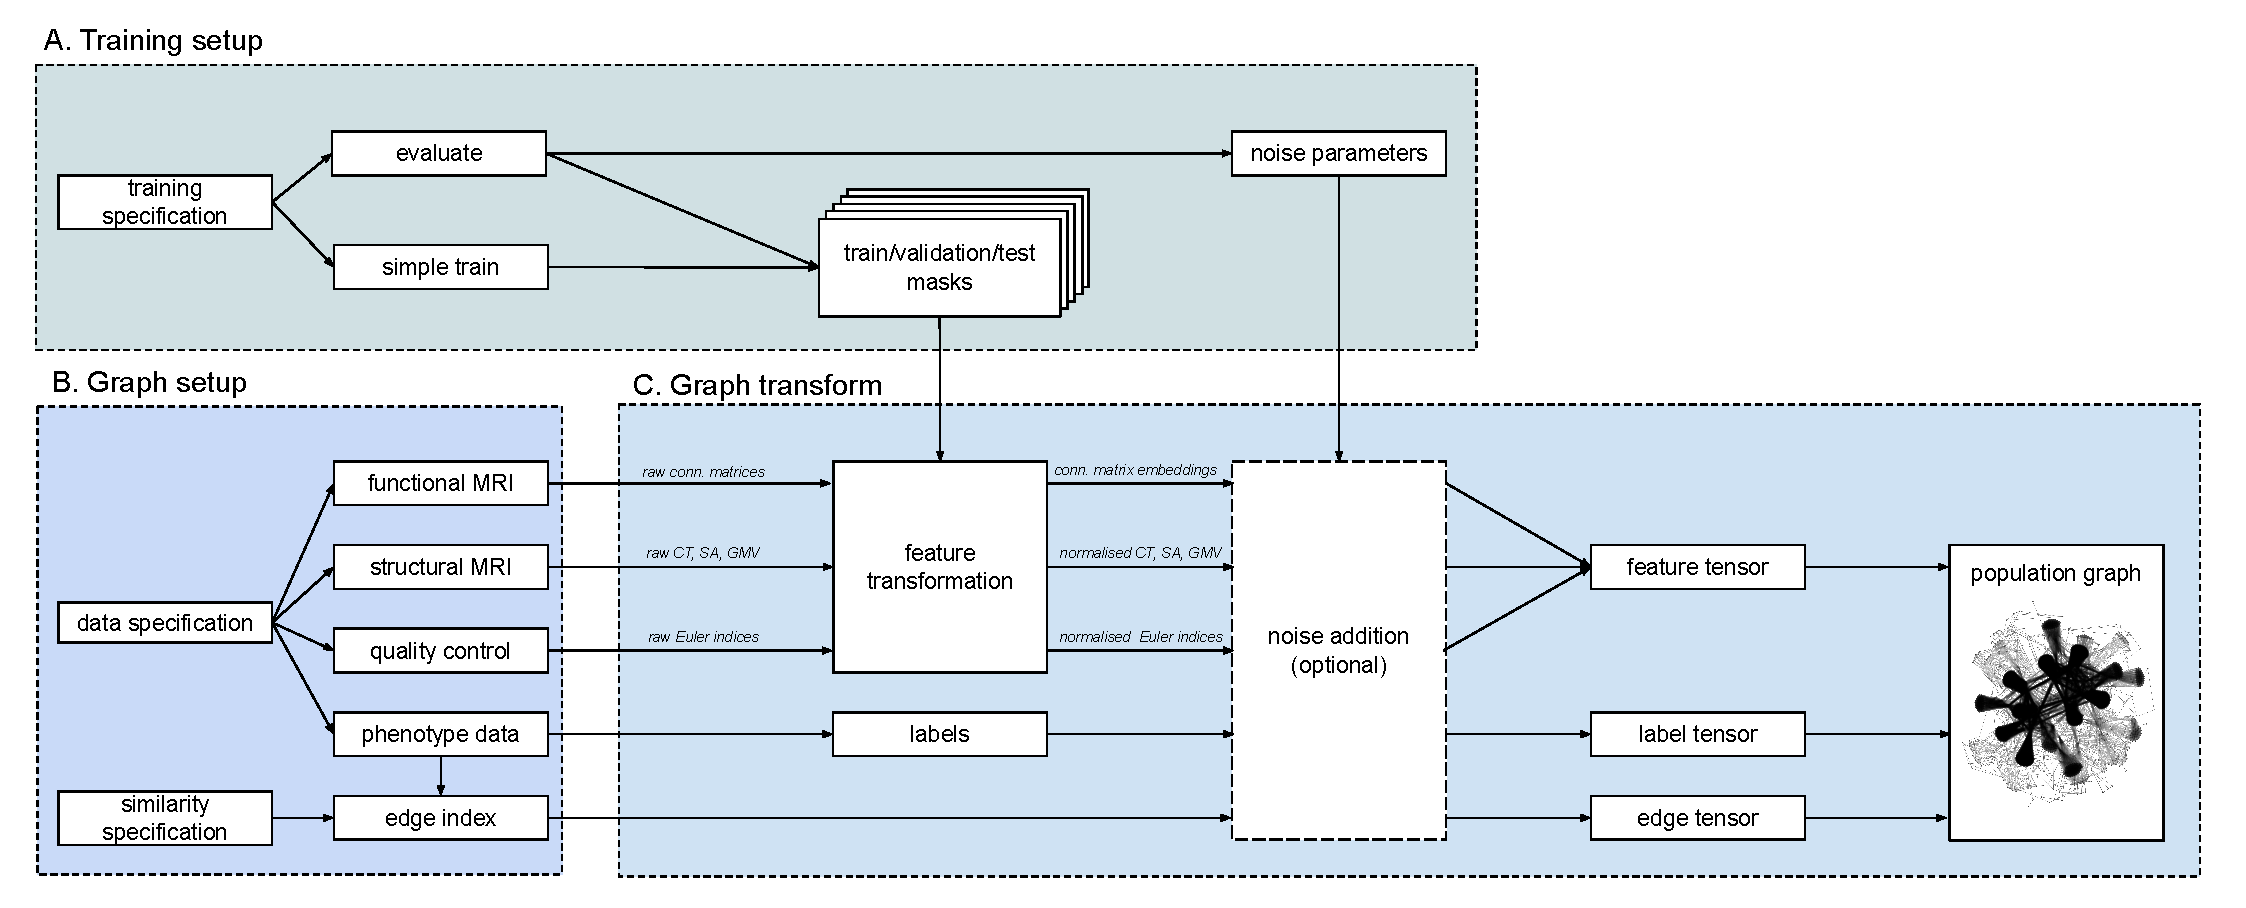
\includegraphics[width=\textwidth]{graphpipeline.pdf}
    \label{graphpipeline}
    \caption{Graph pipeline.}
\end{figure}

\section{Data preprocessing framework}
\subsection{UK Biobank subject selection}
Selecting the subset of subjects that has all data modalities available: some modalities (e.g. phenotypic data) were unavailable because the subjects retracted the permissions to use their data and were removed from the UK Biobank.

Three subjects with inconsistent functional MRI imaging data with some of the regions absent were discarded.


\subsection{Functional connectivity matrix precomputation}

\subsubsection{Dimensionality reduction for neural networks}
The full flattened functional connectivity matrix has over 75,000 features per patient, which, considering pairwise similarities and a large number of subjects, makes the graph (and the training on it) very large: the number of resulting training parameters runs out of memory even for small architectures.

The easiest solution mitigating this is running a PCA on the matrix, assuming that the first few principal components (how many?) would give a good representation of functional data features. Preliminary runs on small datasets of a few thousand subjects give similar performance.

\subsection{Phenotypic data lookup table}
For faster and more convenient similarity matrix precomputation.

One feature in the UK Biobank might be described using several feature IDs corresponding to their versions (or in case of mental health/diagnosis, the indication whether a subject has a particular disorder). Some subjects might have 

Testing.

\subsection{Similarity matrix precomputation}
\textit{Initially considered straightforward pairwise similarities but on the full dataset this proved to be computationally infeasible (estimated runtime over 85 hours just for the mental health similarity)}

Give the maths of how the similarities were vectorised and accelerated using GPUs.

Testing.

\section{Graph construction framework}
This framework accounts for the graph construction once the set of subjects, data modalities, similarity functions and similarity threshold are specified.


\subsection{Similarity function specification}
With \textit{extension}: custom similarity functions


\subsection{Intermediate graph representation}
Describe the resulting intermediate representation as graph construction pipeline is called with specific graph parameters.

Could here mention the \textit{extension} of having weighted edges where edge features would store raw similarity thresholds.

\subsubsection{Node features}
Stored raw because unclear how they should be normalised until the training parameters are set.

\subsubsection{Edge computation}



\section{Graph transformation framework}
Describe how the graph intermediate representation is changed based on the training transformation parameters (training fold, train/validation/test set split). The intermediate graph is prepared for training by normalising the features based on the train subset, adding train/validation/test set masks to ignore subjects that should not be used for feedback in training, concatenating the multiple modalities into a single feature set.

Subject stratification, removing subjects with too few age occurrences because the data cannot be correctly stratified otherwise.


\section{Graph neural network framework}
Description of architecture: number and size of layers etc.

Could have a diagram.

\subsection{Hyperparameter tuning}
Describe which hyperparameters were tuned using Bayesian optimisation strategy, early stopping, cross-validation etc.


\section{Evaluation framework}
The standard performance metrics $r$ and $r^2$ tracked and logged with training.

Describe the additional graph transformation stages which add noise to node features/edges.


\section{Repository overview}
% The repository overview should be around one page in length and should describe the high-level structure of the source code found in your source code Repository; ... could be implemented as a table with folders/file names and the functionality implemented in those files

